\section{Introduction}\label{sec:intro}
There are many different computation tasks which involve undoing of previously 
performed steps or actions. Consider a computation where the action $a$ causes the action $b$,
written $a<b$, and where the action $c$ occurs independently of $a$ and $b$.
There are three  executions of this computation that preserve \emph{causality},
namely $abc$, $acb$ and $cab$. We note that $a$ always comes before $b$.
There are several conceptually different ways of undoing these actions
\cite{irek2014}. {\em Backtracking}
is undoing in precisely the reverse order in which they happened. So, undo $b$ undo $c$ undo
$a$ is a backtrack of the execution $acb$.
{\em Reversing\/} is a more general form of undoing: here actions can be undone in any
order provided causality is preserved (meaning that causes cannot be undone before effects).
For example, undo $c$ undo $b$ undo $a$ is a reversal of $acb$ for the events $a,b$ 
and $c$ above.


There are networks of reactions in biochemistry, however, 
where actions are undone seemingly \emph{out-of-causal order}.
The creation and breaking of molecular bonds between the proteins involved
in the ERK signalling pathway is a good example 
of this phenomenon ~\cite{Irek2012}. Let us assume for simplicity that the creation of molecular 
bonds is represented by actions $a,b,c$ where, as above, $a<b$ and $c$ is independent 
of $a$ and $b$. In the ERK pathway, the molecular bonds are broken in the following 
order: undo $a$, undo $b$, undo $c$, which seems to undo the cause $a$ before the effect $b$. 

We introduced informally a novel and purely local in character mechanism for undoing
of computation in short papers \cite{merevcomp2015,KU16}. Here, we build a process calculus 
around this mechanism and give it operational semantics.
We then discuss various properties that hold in the calculus. Most importantly, 
we show that out-of-causal order computation can be modelled in the calculus. Hence, in general,
the \emph{causal consistency} property \cite{danos2004ccsr} does not hold. There are reachable states 
that can only be arrived at by a mixture of forward and reverse steps. However, we argue that 
causal consistency holds in a restricted version of our calculus, thus the full calculus is in effect
a ``conceptual'' extension of a causally consistent reversible process calculus. The benefits
of the calculus are shown by modelling hydration of formaldehyde 
in water. The molecules of formaldehyde and water are modelled as compositions 
of carbon, oxygen and hydrogen atoms. When composed in parallel, the molecules react 
and the reactions are represented by sequences of transitions of \emph{concerted actions}. 
We are able to represent different forms of reversibility, including out-of-causal order 
reversibility, and computation can proceed in any directions without external control.

The novel features of our calculus are introduced via an example of a simple catalytic reaction.
Consider two molecules $A$ and $B$ that are only able to bond if assisted by a catalyst $C$. 
Once $A$ and $B$ are bonded with the catalyst $C$, $A$ bonds with $B$ and, at the same time, 
the bond between $A$ and $C$ is broken. Finally, the bond between $B$ and $C$ is broken. 
This is illustrated below.
% The reaction steps are shown in Figure~\ref{fig:intro}.

\begin{figure}[h!]
\psfrag{A}{$A$}
\psfrag{B}{$B$}
\psfrag{C}{$C$}
\psfrag{c}{$c$}
\psfrag{d}{$d$}
\psfrag{q}{$q$}

  \centering
    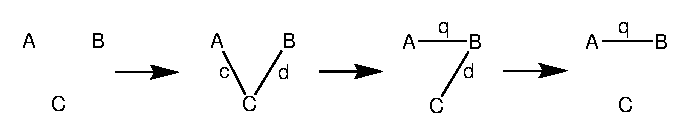
\includegraphics[width=0.8\textwidth]{exampleintro}
  \caption{A catalytic reaction.}
  \label{fig:intro}
\end{figure}

We assume $A  \bydef  (a;p).A'$, $B  \bydef  (b,p).B'$ and $C \bydef  (a,b).C'$, where
$A',B'$ and $C'$ represent further potential behaviour of the molecules $A,B$ and $C$.
%\Stefan{Note that we write the process name with a $'$ instead of $\Nil$ for easy identification of 
%processes without implying any semantical change.} 
We use a new prefix operator $(s;p).P$ where $s$ is a sequence of actions or executed
actions and $p$ is a \emph{weak} action. Initially the actions in $s$ take place, and then $p$ takes place.
%and then we compute with $P$.  
The molecules $A,B$ and $C$ can bond by performing synchronously the
matching actions according to the communication function $\gamma(a,a)=c$, $\gamma(b,b)=d$ and
$\gamma(p,p)=q$, producing thus new actions $c,d$ and $q$ respectively. A weak action $p$ can be left out
in $(s;p)$ 
resulting in the simple prefix $(s).P$ (as in $B$ and $C$ above).
In general, the actions of $s$ in $(s;p).P$ can take place in any order, very much like in
\cite{Danos2007ccsr,Irek2012}, and the new feature is that $p$ can happen only if
all actions in $s$ have already taken place. Once $p$ takes place, one of the executed
actions in $s$ must be undone immediately: this is our new mechanism for
triggering reverse computation.  We shall model these two almost simultaneous
events as a transition of concerted actions. This is a realistic representation of the mechanism 
of covalent bonding, 
the most common type of chemical bonding between atoms, hence we call our calculus
a \emph{Calculus of Covalent Bonding}.

Returning to our example, we represent the system of molecules $A,B$ and $C$ as 
$((a;p).A' \paral (b,p).B' \paral (a,b).C') \setminus \{a,b,p\}$, 
where `$\paral$' is the parallel composition and `$\setminus$' the restriction as in
ACP \cite{BaetenBook}.
We note that $A$ and $B$ cannot interact initially since $\gamma(a,b)$ is not defined. 
They can however both 
interact with $C$:
\begin{flalign*}
&(a;p).A' \paral (b,p).B' \paral (a,b).C' \xrightarrow{c[1]} (a[1];p).A' \paral (b,p).B' 
	\paral (a[1],b).C' \xrightarrow{d[2]} \\
&(a[1];p).A' \paral (b[2],p).B' \paral (a[1],b[2]).C'
\end{flalign*}
Numbers 1 and 2 are the \emph{communication keys} \cite{PhillipsUlidowski06,Irek2007}: they indicate 
which pairs of actions have bonded. 
Molecules $A$ and $B$ can now bond on $p$ (with the key 3), producing the action $q[3]$. 
This causes immediately the breaking of the bond $c[1]$, which means undoing of 
the action $a$ in $A$ and action $a$ in $C$ (and still leaving $A$ and $B$ bonded). 
We model such an event of creating a bond and simultaneously breaking another bond by a
pair of \emph{concerted actions}:
\begin{flalign*}
	&(a[1];p).A' \paral (b[2],p).B' \paral (a[1],b[2]).C' \xrightarrow{\{q[3],\underline{c}[1]\}}\\
       &  (a;p[3]).A' \paral (b[2],p[3]).B' \paral (a,b[2]).C'
\end{flalign*}
The bond with the key 3 on the weak action $p$ in $A$ is unstable, and thus gets \emph{promoted} to 
a stable and stronger 
bond on $a$ and $p$, which is modelled by the following rewrite:
\begin{flalign*}
&(a;p[3]).A' \paral (b[2],p[3]).B' \paral (a,b[2]).C' \Rightarrow (a[3];p).A' \paral (b[2],p[3]).B' 	\paral (a,b[2]).C'
\end{flalign*}
Finally, the catalyst dissolves the bond with $B$:
\begin{flalign*}
(a[3];p).A' \paral (b[2],p[3]).B' \paral (a,b[2]).C'
\xrightarrow{\underline{d}[2]} (a[3];p).A' \paral (b,p[3]).B' \paral (a,b).C'
\end{flalign*}
We note that $A$ and $B$ are now bonded although the synchronisation function did not allow 
it to happen initially. The main consequence of this is that the bond between $a[3]$ and $p[3]$ is 
\emph{irreversible}, namely it cannot be undone.
Looking at the pattern of doing and undoing of bonds we obtain $c[1] d[2] 
q[3] \underline{c}[1] \underline{d}[2]$. Since creation of bonds $c$ and $d$ causes the bond $q$, 
we have here an example of an out-of-causal order computation.

The calculus CCB is given \emph{Structural Operational Semantics} (SOS for short)
style semantics. This includes
novel SOS rules for concerted actions and three rewrite rules that prescribe when bonds on weak actions 
can be promoted to strong action bonds. We show that CCB is a well behaved calculus by proving
a number of useful properties. For example, the sub-calculus with the simple prefixing operator
$(s).P$ satisfies causal consistency. We show that the full calculus allows us to represent 
out-of-causal order computation patterns via the hydration of formaldehyde in water case study. 

Next we summarise the main items of related work.

\subsection{Related Work}

Scientists started to investigate the speed of chemical reactions and the rates achieved as soon as 
the concept of chemical reactions was first developed. The behaviour of a system of compounds over 
time can be modelled using a set of ordinary differential equations (ODEs). The fast calculations 
of such ODEs were popularised by Gillespie \cite{Gillespie} in order to show the dynamic behaviour 
of systems of chemical compounds. When biochemical processes, which involve not only small molecules 
but also macromolecules, cells and membranes, were modelled attention turned to how
the individual objects were represented and how they behaved, and the usefulness of computer 
science methods was demonstrated in \cite{fontana}.

Process calculi are very successful formalisms for representing concurrent and distributed
systems. Each component of a system has its definition which specifies what it does and how it 
interacts with other components. The behaviour of the system emerges then from the independent
actions of the components and from the interactions between them.
Calculus of Communicating Systems (CCS) \cite{Milner1980}, Communicating Sequential Processes (CSP) 
\cite{HoareBook}, and the $\pi$-calculus \cite{MilnerPi} are examples of process calculi.
Starting with Regev et al. \cite{regev2001a,regev2001b,regev2004} process calculi, specifically 
the $\pi$-calculus, were used to model biochemical systems. The biochemical compounds  
are represented as processes, and how they react is modelled by communication on ports. A creation
of a bond or a dissolution of a bond is represented as establishing or breaking of a communication
between ports. 
So there is a natural analogy between concurrent processes and biochemical entities in natural 
systems, and between communication among processes and reactions between biochemical entities.
The aim of this work, as stated in \cite{regev2001b}, was to represent suitably biological knowledge in 
processes and to enable computer-based analysis of this representation. This approach was extended
shortly afterwards to include reaction rates \cite{PriameRegev} using the stochastic $\pi$-calculus, 
which was introduced previously in \cite{PriamiStochasticPi}.

Various other calculi, including  Bio-PEPA (\cite{CiocchettaBiopepa}), the biochemical abstract 
machine (BIOCHAM, \cite{biocham}), P systems (\cite{psystems}), BioAmbients (\cite{RegevBioambients}), 
the kappa calculus (\cite{danos2004kappa}) and Brane Calculus (\cite{CardelliBraneCalculi}),
followed aiming to capture various other aspects of biological systems such as,
for example, compartments and  membranes.

Most of biochemical reactions are reversible, and creating bonds is as important in biochemical processes
as breaking of bonds. Hence, it became useful to be able to represent directly reversibility in
process calculi. This realisation lead to the development of a number of reversible
process calculi \cite{danos2004ccsr,Danos2007ccsr,PhillipsUlidowski06,Irek2007,LaneseMS10,Lanese_controllingreversibility,Lanese_controlled,CKV13}, which have application far beyond biochemistry.
Out-of-causal order reversibility, an important aspect of biochemical system which is
typically not captured in traditional reversible process calculi, was first proposed 
in \cite{Irek2012}, where the calculus CCSK 
\cite{Irek2007} is extended with an \emph{execution control mechanism} for 
managing the pattern and the direction of computation. The control mechanism for reversibility
is external to the processes it controls, and it can have a global scope. The calculus introduced 
in this paper has in contrast  no global control and the behaviour
of a biochemical systems emerges from the behaviour of its components. Out-of-causal order computation
was also studied in \cite{Irek2013,irekconcur2013}.

\section{A Calculus of Covalent Bonding}\label{sec:calculus}

In this section we define the calculus introduced informally in the Introduction. 
First, we introduce some preliminary notions and notations.

Let $\mA$ be the set of (forward) action labels, 
ranged over by $a,b,c,d,e,f$. We partition $\mA$ into the set of \emph{strong actions}, written as
$\mSA$, and the set of \emph{weak actions}, written as $\mWA$. Reverse (or past) action labels are members of
$\underline\mA$, with typical members $\un{a},\un b, \un c,\un d, \un e ,\un f$, and represent 
undoing of actions. The set $\mathcal{P}(\mA \cup \underline\mA)$ is ranged over by $L$.

Let $\Keys$ be an infinite set of {\em communication keys} (or {\em keys} for short)
\cite{PhillipsUlidowski06,Irek2007}, ranged over by $k,l, m,n$. The Cartesian product $\mathcal A \times \Keys$, denoted by $\mAK$,
 represents past actions, which are written as $a[k]$ for $a\in \mA$ and $k\in\Keys$. 
Correspondingly, we have the set $\umAK$ that represents undoing of past actions. We use $\alpha, \beta$ to identify actions which are either from $\mA$ or $\mAK$. It would be 
useful to consider sequences of actions or past actions, namely the elements of $(\mA \cup \mAK)^*$, 
which are ranged over by $s,s'$ and sequences of purely past actions, namely the elements of $\mAK^*$, 
which are ranged over by $t,t'$. The empty sequence is denoted by $\epsilon$. We use the notation $\alpha, s$ and
$s,s'$ to denote a concatenation of elements, which can be strings or single actions.

We shall also use two sets of auxiliary action labels, namely the set $(\mA) =\{ (a)\ \mid a\in\mA\}$, and its product with the set of keys, namely $(\mA)\Keys$. These labels will be used in the auxiliary rules when defining
the semantics of CCB.

We now define the Calculus of Covalent Bonding, or CCB for short. The syntax of CCB is given 
below where $P$ is a process term:

$$P ::=  S \ \mid \ (s;b).P \ \mid \ P\paral Q \ \mid \ P\restrict L $$

The set of process identifiers (constants) $\PI$ contains typical elements $S$ and $T$. 
A process identifier $S$ has normally a defining equation $S\bydef P$ where $P$ contains only forward 
actions (and no past actions). There is also a special identifier
 $\Nil$, denoting the deadlocked process, which has no defining equation.

We have a general prefixing operator
$(s;b).P$, where $s$ is a non-empty sequence of actions or past actions. This operator
extends the prefixing operator in \cite{Irek2012}. The action $b$ is a weak action
and it can be omitted, in which case the prefixing is written as $(s).P$ and is called the
\emph{simple prefix}. The simple prefix is the prefixing operator in \cite{Irek2012}. 
One of the actions in $s$ in $(s).P$ may be a weak action from $\mWA$. If $s$ is a sequence that contains   
a single action, then the action is a strong action and the operator 
is the prefixing operator of CCS \cite{Milner1980}.
We omit trailing $\Nil$s so, for example, $(s).\Nil$ is written as $(s)$.
%
% Move this example to somewhere later
%
\Comment{\Stefan{We will only use cases in this paper where processes are of the form $(s).\Nil$. We still have the possibility of 
processes like $(s).(s').\Nil$ in our calculus. This could be used to model protein functions in biological systems, for example 
base excision repair (\cite{Köhler2014}. For this a protein ``walks'' along a strand of DNA and repairs faults which occurred in 
DNA replication. Such a protein could be modelled by having the walk modelled in $s$ and the repair mechanism in $s'$, combining them to a model like $(s).(s').\Nil$.}
}
%
%
The new feature of the operator $(s;b).P$ is the execution of the weak action $b$, which
can happen only after all the actions in $s$ have taken place. Performing $b$ then forces
undoing one of the past actions in $s$ (by the \rulename{concert} rule in Figure~\ref{fig:csos}).

$P\paral Q$ represents two systems $P$ and $Q$ which can perform actions or reverse actions on
their own, or which can interact with each other according to a communication function
$\gamma$. As in the calculus ACP \cite{ACPBook}, the communication function is a partial function 
$\gamma: \mathcal A \times \mathcal A \rightarrow \mathcal A$ which is commutative and associative. The function
$\gamma$ is used in the operational semantics to define when two processes can interact. Processes 
$P$ and $Q$ in $P\paral Q$ can also perform a pair of concerted actions,
which is the new feature of our calculus.  We also have the ACP-like restriction operator 
$\setminus L$, where $L$ is a set of labels. It prevents actions from taking place and, due to 
the synchronisation algebra used, it also blocks communication. If $\gamma(a,b)=c$ then $a.P$ and $b.Q$
cannot communicate in $(a.P\paral b.Q)\setminus c$.
Note that we do not use here the usual relabelling 
operator $[f]$, where $f: \mA \rightarrow \mA$, which could be easily added.

%
%move this elsewhere?
%
The example in the Introduction and our main example in Section~\ref{sec:bigexample} seem to indicate that only
simple processes of the form $(s;b).\Nil$ are sufficient in the modelling of chemical reactions. 
However, there are examples where a nested prefix $(s;b).(s';b').P$ is useful. 
Consider a base excision repair as in \cite{Köhler2014} where a protein ``walks'' along 
a strand of DNA and repairs faults which occurred in the DNA replication. The walking along a DNA strand 
could be modelled by actions in $s$, and, once a fault is found, the repair mechanism could be modelled
by the actions in $s'$. Another example where the full calculus is useful is a model of long 
standing transactions with compensations in \cite{Irek2012}.


The set of \emph{process terms} is ranged over by $P,Q$ and $R$ and is denoted by $\Proc$. 
In the setting of CCB these terms are called simply \emph{processes}. 
A context $C\hole$ is a process term containing a \emph{hole}, represented by $\hole$. 
Formally, contexts are defined by
the following syntax: $C::= \hole \mid (s;b).C \mid P\paral C \mid C \paral P \mid C\restrict L $.
The term $C[Q]$ denotes the result of filling the hole in the context $C\hole$ with the process $Q$.
We say that $R$ is a \emph{subprocess} of $P$ if $P$ is $C[R]$ for some context $C\hole$.

We define the semantics of our calculus by a labelled transition system,
LTS for short, which is a structure $(St,AL,\rightarrow: \subseteq St \times AL \times St)$
with $St$ the set of states, $AL$ the set of action labels and $\rightarrow: 
\subseteq St \times AL \times St$ the labelled transition relation.
The set of states $St$ is the set $\Proc$. In practice, all our results and examples hold for
\emph{consistent} processes, namely processes
reachable from standard processes (see Definition~\ref{consistent}). 
The action labels are the forward actions $\mAK$, 
the reverse actions $\umAK$ and the \emph{pairs of concerted actions} $\mAK \times \umAK$. 
%
The labelled transition relation is defined by SOS rules (Figures~\ref{fig:fsos}--\ref{fig:sc}) 
and rewrite rules (Figure~\ref{fig:reduction}), where
the rules in Figures~\ref{fig:fsos}--\ref{fig:reversesos}
are influenced by \cite{Irek2007}. 
Note that
sequences $s$ and $t$ are members of $(\mathcal{A}\cup\mathcal{AK})^*$ and $\mathcal{AK}^*$
respectively in Figures~\ref{fig:fsos}--\ref{fig:csos}.

We now introduce and explain the SOS rules before returning to 
the rewrite rules. Let $r$ be an SOS rule for an operator $f$ of CCB as in 
Figures~\ref{fig:fsos}--\ref{fig:csos}. 
%Then, $f$ is the operator of $r$ and the elements of $X$ are the arguments of $r$. 
%We write $rules(f)$ for the set of SOS rules for $f$. 
Transitions above the horizontal bar in $r$ are called \emph{premises}. 
The set of premises is written as
$pre(r)$. The transition below the bar in $r$ is the $\emph{conclusion}$ and 
is written as $con(r)$. 
%
\begin{figure}[t] 
\[
\begin{array}{ll}
\Rule
{}
{\std{\Nil}}
\qquad &
\Rule
{}
{\fresh{m}{\Nil}}
\\[15pt]
\Rule
{\std{P}}
{\std{S}}
\quad
S \bydef P
\qquad &
\Rule
{\fresh{m}{P}}
{\fresh{m}{S}}
\quad
S \bydef P
\\[15pt]
\Rule
{\kkey{s}=\emptyset \quad  \std{P}}
{\std{(s;b).P}}
\qquad &
\Rule
{m \notin \kkey{s} \quad \fresh{m}{P}}
{\fresh{m}{(s;b).P}}
\\[15pt]
\Rule
{\std{P} \quad \std{Q}}
{\std{P \paral Q}}
\qquad &
\Rule
{m \notin \kkey{s} \quad m \neq n \quad \fresh{m}{P}}
{\fresh{m}{(s;b[n]).P}}
\\[15pt]
\Rule
{\std{P}}
{\std{P \setminus L}}
\qquad &
\Rule
{\fresh{m}{P} \quad \fresh{m}{Q}}
{\fresh{m}{P \paral Q}}
\qquad 
\Rule
{\fresh{m}{P}}
{\fresh{m}{P \setminus L}}
\end{array}
\] 
\caption{Predicates $\mathsf{std}$ and $\mathsf{fsh}$.} 
\label{fig:predicates}
\end{figure}
%
We use two predicates $\std{P}:\Proc$ and $\fresh{m}{P}:\Keys \times \Proc$ in our SOS rules. 
They are defined in Figure~\ref{fig:predicates}, and they use two auxiliary functions
$\kkey{s}: (\mathcal{A}\cup\mathcal{AK})^* \rightarrow \mathcal{P}(\Keys)$ and
$\keys{P}: \Proc \rightarrow \mathcal{P}(\Keys)$. 
The function $\kkey$ is defined as follows:
$\kkey{\epsilon}=\emptyset$, $\kkey{\alpha:s}=\{l\}\cup\kkey{s} \text{ if }\alpha=a[l]$, for 
$a\in \mathcal{A}$ and $l\in \Keys$, and $\kkey{\alpha:s}= \kkey{s} \text{ if }\alpha \in \mathcal{A}$.
The function $\keys$ is given by $\keys{\Nil}=\emptyset$, $\keys{S}=\keys{P}$ if $S\bydef P$, $\keys{(s;b).
P}=\kkey{s} \cup \kkey{b} \cup \keys{P}$, $\keys{P \paral Q}= \keys{P} \cup \keys{Q}$, and $\keys{P \restrict L}=\keys{P}$. Informally $\keys{P}$ associates with each term $P$ the set of its keys. 
A process $P$ is standard, written $\std{P}$, if it contains no past actions (hence no keys). 
A key $n$ is fresh in $Q$, written $\freshpred{n}(Q)$, if $Q$ contains no past action with the key $n$.
We extend the notion of fresh keys to the sequences of actions and past actions $s$ and $t$ 
via the function $\kkey$.
%Figure~\ref{fig:predicates} defines the predicates by induction over the process terms. 
%We could also have said that $\std{P}$ is true if $\keys{P} = \emptyset$ and that 
%$\fresh{m}{P}$ is true if $i \notin \keys{P}$.

\begin{figure}[t] 
\[
\begin{array}{ll}
\rulename{act1}\ 
\Rule
{\std{P} \quad \fresh{k}{s,s'}}
{(s,a,s';b).P \xrightarrow{a[k]}(s,a[k],s';b).P}
\qquad &
\rulename{act2}\
\Rule
{P \xrightarrow{a[k]} P' \quad \fresh{k}{t}}
{(t;b).P \xrightarrow{a[k]} (t;b).P'}
\\[25pt]
%\rom{act3}\ Dec 17
%\Rule
%{\std{P} \quad \fresh{k}{t,t'}}
%{(t,b,t';b').P \xrightarrow{b[k]}(t,b[k],t';b').P}
%\qquad &
%\\[25pt]
\rulename{par}\
\Rule
{P \xrightarrow{a[k]} P'\quad \fresh{k}{Q}}
{P \paral Q \xrightarrow{a[k]} P' \paral Q}
\qquad &
\rulename{com}\
\Rule
{P \xrightarrow{a[k]} P' \quad Q \xrightarrow{d[k]} Q'}
{P \paral Q \xrightarrow{c[k]} P' \paral Q'}
\; (*)
%
\\[25pt]
\rulename{res}\
\Rule
{P \xrightarrow{a[k]} P'}
{P\backslash L \xrightarrow{a[k]} P'\backslash L}
\; a \notin L
\qquad &
\rulename{con}\
\Rule
{P \xrightarrow{a[k]} P'}
{S \xrightarrow{a[k]} P'}
\; S \bydef P
\end{array}
\] 
\caption{Forward SOS rules. The condition (*) is $\gamma(a,d)=c$, 
and $b \in \mathcal{WA}$.} \label{fig:fsos}
\end{figure}
\begin{example}
{\rm
We illustrate how processes compute forwards using the new prefixing operator. Consider a standard
process $(a;b).(c) \paral (a,d,c)$ and the communication function $\gamma$ given by $\gamma(a,a)=a$ 
and $\gamma(c,c)=c$. We have
$$(a;b).(c) \paral  (a,d,c) \xrightarrow{a[1]} (a[1];b).(c) \paral  (a[1],d,c)$$
by the SOS rules \rulename{act1} and \rulename{com} from Figure~\ref{fig:fsos}. This is because $(c)$ 
is standard and the key 1 is fresh in $\varepsilon$. The next step of computation involves a communication of
the actions $c$, which we obtain by rules \rulename{act2} and \rulename{com}:
$$(a[1];b).(c) \paral  (a[1],d,c) \xrightarrow{c[2]} (a[1];b).(c[2]) \paral  (a[1],d,c[2])$$
We note that the key 2 is fresh in $a[1]$. Finally, the action $d$ takes place by \rulename{act1} and,
informally, the symmetric version of \rulename{par}.
$$(a[1];b).(c[2]) \paral  (a[1],d,c[2]) \xrightarrow{d[3]} (a[1];b).(c[2]) \paral  (a[1],d[3],c[2])$$
Formally, we use \rulename{par}, the structural congruence rule \rulename{sc} in Figure~\ref{fig:sc}
and the reduction rule \rulename{red1} in Figure~\ref{fig:reduction}.
}
\end{example}

\begin{figure}[t]
\[
\begin{array}{ll}
\rulename{rev act1}\
\Rule
{\std{P} %\quad \fresh{k}{s,s'}
}
{(s,a[k],s';b).P \xrightarrow{\underline{a}[k]}(s,a,s';b).P}
\quad &
%
% b was previously beta. Since we must apply prom rewrite before we apply any SOS rule, we do not 
% need a rule with a beta.
%
% referees suggested to remove fsh predicates from both act rules. They were there for symmetry reason 
% with the forward rules but are not used in the reverse.
%
\rulename{rev act2}\
\Rule
{P \xrightarrow{\underline{a}[k]} P' %\quad \fresh{k}{t}
}
{(t;b).P \xrightarrow{\underline{a}[k]} (t;b).P'}
\\[25pt]
% Dec 17
%\rom{rev act3}\
%\Rule
%{\std{P}  \quad \fresh{k}{t,t'} }
%{(t,b[k],t';b').P \xrightarrow{\underline{b}[k]} (t,b,t';b').P'}
%& \\[25pt]
\rulename{rev par}\
\Rule
{P \xrightarrow{\underline{a}[k]} P'\quad \fresh{k}{Q}}
{P \paral Q \xrightarrow{\underline{a}[k]} P' \paral Q}
\quad &
\rulename{rev com}\
\Rule
{P \xrightarrow{\underline{a}[k]} P' \quad Q \xrightarrow{\underline{d}[k]} Q'}
{P \paral Q \xrightarrow{\underline{c}[k]} P' \paral Q'}
\; (*)
%
\\[25pt]
\rulename{rev res}\
\Rule
{P \xrightarrow{\underline{a}[k]} P'}
{P\backslash L \xrightarrow{\underline{a}[k]} P'\backslash L}
\; a \notin L
\quad &
\rulename{rev con}\
\Rule
{P \xrightarrow{\underline{a}[k]} P'}
{P \xrightarrow{\underline{a}[k]} S}
\; S \bydef P'
\end{array}
\]
\caption{Reverse SOS rules. The condition (*) is $\gamma(a,d)=c$, and 
and $b \in \mathcal{WA}$. %Note that $\beta \in \mA \cup \mAK$.
} 
\label{fig:reversesos}
\end{figure}

\begin{figure}[t] 
\[
\begin{array}{l}
\rulename{aux1}\ 
\Rule{\std{P} \quad \fresh{k}{t}}
{(t;b).P \xrightarrow{(b)[k]}(t;b[k]).P}
\qquad
\rulename{aux2}\
\Rule
{P \xrightarrow{(b)[k]} P' \quad \fresh{k}{t}}
{(t;b').P \xrightarrow{(b)[k]} (t;b').P'}
\\[25pt]
\rulename{concert}\ 
\Rule
{P\xrightarrow{(b)[k]}P' \quad P'\xrightarrow{\underline{a}[l]}P'' \qquad Q\xrightarrow{\alpha[k]}Q' 
  \quad Q'\xrightarrow{\underline{d}[l]}Q''% %\quad \fresh{k}{Q} 
 }
{P \paral Q\xrightarrow{\{e[k],\underline{f}[l]\}} P'' \paral Q''} (*)\\[25pt]
\rulename{concert act}\
\Rule
{P \xrightarrow{\{{a}[k], \underline{h}[l]\}} P' \quad \fresh{k}{t}}
{(t;b).P \xrightarrow{\{{a}[k], \underline{h}[l]\}} (t;b).P'}\\[25pt]
\rulename{concert par}\
\Rule
{P \xrightarrow{\{{a}[k], \underline{h}[l]\}} P'\quad \fresh{k}{Q} \quad \fresh{l}{Q}}
{P \paral Q \xrightarrow{\{{a}[k], \underline{h}[l]\}} P' \paral Q}\\[25pt]
\rulename{concert res}\
\Rule
{P \xrightarrow{\{{a}[k], \underline{h}[l]\}} P'}
{P\backslash L \xrightarrow{\{{a}[k], \underline{h}[l]\}} P'\backslash L} (**)
%
\end{array}
\] 
\caption{SOS rules for concerted actions. The condition (*) is 1. $\alpha$ is $c$ or $(c)$ 
and $\gamma(b,c)=e$ for some $c\in \mathcal{A}$, and 2. $\gamma(a,d)=f$. 
The condition (**) is $a, \underline{h}  \notin L \cup (L)$. 
Recall that $t \in \mAK^*$.} \label{fig:csos}
\end{figure}

\begin{figure}[t] 
\[
\begin{array}{l}
%\rom{sc}\
\Rule
{P \Rightarrow Q \quad Q \tran{\mu} Q' \quad Q' \Rightarrow P'}
{P\tran{\mu} P'} 
%\quad \mu \in \mAK\cup \umAK \cup \mathcal{C}
%%TODO Moreover, $S\equiv P$ for all $S, P$ 
%%such that $S\bydef P$.
\end{array}
\] 
\caption{Structural congruence rule sc when $\mu\in \mAK \cup (\mAK\times \umAK)$,
and rev sc when $\mu\in \umAK$.} 
\label{fig:sc}
\end{figure}

\begin{figure}[t] 
\[
\begin{array}{lll}
\rulename{red1}: & P\Par Q \Rightarrow Q\Par P& 
\\[10pt]
\rulename{red2}: & P\Par (Q\Par R) \Rightarrow (P\Par Q)\Par R &
\\[10pt]
\rulename{red3}: & (P\Par Q)\Par R \Rightarrow P\Par (Q\Par R) & 
\\[10pt]
\rulename{red4}: & P\Par \Nil \Rightarrow P & 
\\[10pt]
\rulename{red5}: & (P\paral Q)\backslash L \Rightarrow P\backslash L \paral Q & \mbox{ if fn(Q)} \cap L = \emptyset
\\[10pt]
\rulename{red6}: & P\backslash L \paral Q \Rightarrow (P\paral Q)\backslash L & \mbox{ if fn(Q)} \cap L = \emptyset
\\[10pt]
\rulename{prom}: & (s,a,s';b[k]).P \Rightarrow (s,a[k],s';b).P & \mbox{ if } a \in \mathcal{SA}, b \in \mathcal{WA} 
\\[10pt]
\rulename{move-r}: & (s,a,s',b[k],s'').P \Rightarrow (s,a[k],s',b,s'').P & \mbox{ if } a \in \mathcal{SA}, b \in \mathcal{WA}
\\[10pt]
\rulename{move-l}: & (s,b[k],s',a,s'').P \Rightarrow (s,b,s',a[k],s'').P & \mbox{ if } a \in \mathcal{SA}, b \in \mathcal{WA}
\end{array}
\] 
\caption{Reduction rules. Sequences $s, s', s''$ are members of $(\mathcal{A} \cup \mathcal{AK})^{*}$.} 
\label{fig:reduction}
\end{figure}

The next example illustrates how some of the reverse SOS rules work.
\begin{example}
{\rm 
Consider $(a[1],b).(c).S$ where $S\bydef (a,b).(c).S$. We have 
$$(a[1],b).(c).S \xrightarrow{\underline{a}[1]} (a,b).(c).S$$ by \rulename{rev act1} since $(c).S$ is standard.
Since $(a,b).(c).S$ is the definition of $S$ we obtain by rule \rulename{rev con} $(a[1],b).(c).S \xrightarrow{\underline{a}[1]} S$.
}
\end{example}

Figure \ref{fig:csos} contains the SOS rules that define the new concerted actions transitions. 
The main rule is the rule \rulename{concert} that defines when a pair of concerted actions 
takes place.  We also have two auxiliary rules \rulename{aux1} and \rulename{aux2} which 
define only an auxiliary transition relation needed in the \rulename{concert} rule. 
Note that the \rulename{concert} rule uses \emph{lookahead} \cite{Uli92}.
Also note that transitions in \rulename{aux1} and \rulename{aux2} use the auxiliary labels $(b)[k]$ 
for all $b \in \mWA$ and $k \in \Keys$. The rule \rulename{concert par} requires that $k$ is fresh in $Q$,
correspondingly as in \rulename{par}. Moreover, we need to ensure that when we reverse $h$ with the key $l$
in $P$ we do not leave out any actions with the key $l$ in $Q$ which make up a multiaction 
communication with the key $l$. Hence, we also include the premise $\fresh{l}{Q}$ in \rulename{concert par}.
The rule \rulename{concert act} requires, correspondingly as \rulename{act}, that $k$ is fresh in $t$.
Our operational semantics guarantees that if a standard process evolves to $(t;b).P$, for some $P$, and
$P$ reverses an action with the key $l$, then $l$ is fresh in $t$. Hence, we do not include $\fresh{l}{t}$
in the premises of \rulename{concert act}.
%
Next, we illustrate how concerted actions transitions work.

\begin{example}\label{ex:examp1}
{\rm Consider the process $(a;b) \paral a \paral b$ with $\gamma(a,a)=c$ and $\gamma(b,b)=d$. After the
initial synchronisation of actions $a$, which produces the transition $c[1]$, we have a transition
with a pair of concerted actions by rule \rulename{concert} in Figure~\ref{fig:csos}
$$(a[1];b) \paral a[1] \paral  b \xrightarrow{\{d[2], \underline{c}[1]\}} 
  (a;b[2])\paral a \paral b[2]$$
since $(a[1];b) \xrightarrow{(b)[2]} (a[1];b[2])$ by \rulename{aux1}, 
$(a[1];b[2]) \xrightarrow{\underline{a}[1]} (a;b[2])$ by \rulename{rev act1}, 
and since $a[1] \paral b \xrightarrow{b[2]} a[1] \paral b[2] \xrightarrow{\underline{a}[1]} a \paral b[2]$
by \rulename{par} and \rulename{rev par}.}
\end{example}

\begin{example}\label{ex:examp2}
{\rm Consider $(a[1];b)\paral (a[1];b)\paral e$ with $\gamma(a,a)=c$ and $\gamma(b,b)=d$.
We clearly have the following pair of concerted actions
 $$(a[1];b)\paral (a[1];b)\paral e  \xrightarrow{\{d[2], \underline{c}[1]\}} 
(a;b[2])\paral (a;b[2])\paral e. $$}
\end{example}

There are processes with weak actions that can potentially communicate but there are no concerted actions 
transitions due to our SOS rules:

\begin{example}\label{ex:examp3}
{\rm Consider $(a[1];b)\paral (e[2];b)\paral (a[1],e[2])$ with $\gamma(a,a)=c$ and $\gamma(b,b)=d$.
The process cannot perform any concerted actions: Although $(a[1];b)  \xrightarrow{(b)[l]} 
\xrightarrow{\underline{a}[1]} (a;b[l])$, for any $l$ different from 1 and 2, but
$(e[2];b)\paral (a[1],e[2])$  cannot perform the auxiliary $(b[l])$
transition since there are no SOS rules for parallel composition and auxiliary actions $(b)$. This forces us
to treat $(a[1];b)$ and $ (e[2];b)$ as $P$ and $Q$ in the \rulename{concert} rule, respectively, and we notice that
we cannot undo a communication on $a$ or $e$.}
\end{example}

Overall, the transitions in Figures~\ref{fig:fsos}--\ref{fig:csos} are labelled with $a[k] \in \mAK$, or with 
$\underline{c}[l] \in \umAK$, or with concerted actions $(a[k], \underline{c}[l])$.
%\} \in \mathcal{C}$.

We also have the usual structural congruence rules 
sc and rev sc in Figure~\ref{fig:sc}, 
which potentially combine reductions (defined below) with transitions.

Next, we introduce our reduction relation which is given by the reduction (rewrite) rules 
in Figure~\ref{fig:reduction}. The reduction relation is needed to define {\em promotion} 
of actions. First we define the function $\mathsf{fn}$ for {\em free names} of processes.

\begin{definition} \normalfont 
The function $\mathsf{fn}: \Proc \rightarrow \mathcal{P}(\Keys)$ is given as follows: 
$\mathsf{fn}(\Nil) = \emptyset$,
$\mathsf{fn}(S)=\mathsf{fn}(P) \text{ if }  S\bydef P$, $\mathsf{fn}((\alpha : s;b).P)=\{\alpha\} \cup 
\mathsf{fn}((s;b).P)$, $\mathsf{fn}((a;b).P)=\{a,b\} \cup \mathsf{fn}(P) $, $\mathsf{fn}(P\paral Q)=\mathsf{fn}(P) \cup \mathsf{fn}(Q)$, and $\mathsf{fn}(P \restrict L)=\mathsf{fn}(P) \restrict L$.
\end{definition}

\noindent
Our reduction rules have names such as, for example, \rulename{red} and we write 
\rulename{red}: $P \Rightarrow Q$
to indicate that the reduction rule $P \Rightarrow Q$ is called \rulename{red}. 
The process $P$ in the rule
$P\Rightarrow Q$ is called a \emph{redex}, and the process $Q$ is called a \emph{contractum}. 
A reduction rule $P\Rightarrow Q$ can be seen as a prescription 
for deriving rewrites $C[P] \Rightarrow C[Q]$ for arbitrary context $C[\ ]$. 
A $P$ redex may be replaced by its contractum $Q$ in an arbitrary context 
$C[\ ]$ giving rise to a reduction step: $C[P] \Rightarrow C[Q]$.

\begin{definition} \normalfont The reduction relation $\Rightarrow$ is the smallest reflexive and 
transitive relation on CCB processes that is preserved by all contexts, and that satisfies the rules 
in Figure~\ref{fig:reduction}.
\end{definition}
Note that we do not want $\Rightarrow$ to be symmetric as we wish to apply \rulename{prom} only 
from left to right. 

The rewrite rules in Figure~\ref{fig:reduction} include 
\rulename{prom}, \rulename{move-r}, and \rulename{move-l} which  
promote weak bonds (here $b$) to strong bonds (here $a$).
The rule \rulename{prom} applies to the full version of our prefix operator (with the ; construct), and
\rulename{move-r} and \rulename{move-l} apply only to the simple prefix.
These three rules are here to model what happens in chemical systems: a bond on a weak action is 
temporary and as soon as there is a strong action that can accommodate that bond (as the result
of concerted actions) the bond establishes itself on the strong action thus releasing the weak action.
In order to align the use of these three rules to what happens in chemical reactions, we insist
that they are used as soon as they becomes applicable: this is made 
precise in Definition~\ref{LTS}.
We could have used the idea of ordering on SOS rules and rewrite rules \cite{irek2002,mousavi}
to specify that the rewrite rules \rulename{prom}, \rulename{move-r} and \rulename{move-r} are higher 
in the ordering than all SOS rules and the remaining rewrite rules, implying that they should 
be applied first when deriving transitions. Alternatively, we could have tried to 
employ some of the techniques presented in \cite{Cleaveland2001711} to define our transition relation.
This would require the use of negative information in the premisses, and the definitions in the style
as those in \cite{irek2002,mousavi}.  However, since we combine SOS rules
with rewrite rules, we opted for a directly defined transition relation.

We now define the transition relation for the labelled transition system for CCB.
Recall that the states of the LTS are processes in $\Proc$ and the labels are members of $\mA$,
$\mAK$, $\aAK$ and the concerted actions labels in $\mAK \times \umAK$. 
%We shall use this notation.
Let $d:\Proc \rightarrow \mathbb{N}$ be the operator depth function defined by 
$d(P)=0$ if $P$ is a constant, and $d(f(P_1,\ldots,P_n))=1+max\{d(P_i)\vert 1 \leq i \leq n\}$ 
otherwise, where $f$ is an operator of CCB. The transition relation is given as follows:
%
%
\Comment{old definition
\begin{definition}\label{LTS} \normalfont 
We associate to $\Proc$ and $\mAK \cup \umAK \cup \aAK \cup (\mAK \times \umAK)$ 
a transition relation 
$\rightarrow$ given by $ \bigcup_{l<\omega} \rightarrow^l$, where transition relations 
$\rightarrow^l \subseteq \Proc \times \mAK \cup \umAK \cup \aAK \cup (\mAK \times \umAK) \times \Proc$ 
are as follows, with $b\in \mAK$ and $\mu \in \mAK \cup \umAK \cup (\mAK \times \umAK)$:
\begin{enumerate}
%
\item
$P \xrightarrow{(b)[k]} P' \in \rightarrow^l$ if $d(P)=l$, 
$P \xrightarrow{(b)[k]} P'= \rho(con(r))$, for $r$ either \rulename{aux1} or \rulename{aux2} 
and a substitution $\rho$,
and each premise in $\rho(pre(r))$ is a valid transition in $\bigcup_{k<l} \rightarrow^k$ or a valid predicate.

\item $P \tran{\mu} P'\in \rightarrow^l$ if $d(P)=l$, $P\Rightarrow Q$, for some $Q$ such that $Q$ 
does not contain any \rulename{prom}, \rulename{move-r} and \rulename{move-l} redex,  $Q \tran{\mu} Q'= \rho(con(r))$, for some 
rule $r$ and a substitution $\rho$, such that each member of $\rho(pre(r))$ is either a valid transition 
in $ \bigcup_{k<l} \rightarrow^k$, a valid rewrite or a valid predicate, and $Q'\Rightarrow P'$.
\end{enumerate}
\end{definition}
}
%
%
\begin{definition}\label{LTS} \normalfont
We associate to $\Proc$ and $\mAK \cup \umAK \cup \aAK \cup (\mAK \times \umAK)$
a transition relation
$\rightarrow$ given by $ \bigcup_{l<\omega} \rightarrow^l$, where transition relations
$\rightarrow^l \subseteq \Proc \times \mAK \cup \umAK \cup \aAK \cup (\mAK \times \umAK) \times \Proc$
are as follows, with $b\in \mAK$ and $\mu \in \mAK \cup \umAK \cup (\mAK \times \umAK)$:

\begin{enumerate}
\item
$P \xrightarrow{(b)[k]} P' \in \rightarrow^l$ if $d(P)=l$,
$P \xrightarrow{(b)[k]} P'= \rho(con(r))$, where $r$ is either \rulename{aux1} or \rulename{aux2},
and each premise in $pre(r)$ is a valid transition in $\bigcup_{k<l} \rightarrow^k$ or a valid predicate.

\item $P \tran{\mu} P'\in \rightarrow^l$ if $d(P)=l$, $P\Rightarrow Q$, for some $Q$ such that $Q$
does not contain any \rulename{prom}, \rulename{move-r} and \rulename{move-l} redex,  $Q \tran{\mu} Q'= con(r)$,
for some rule $r$ where each member of $pre(r)$ is either a valid transition
in $ \bigcup_{k<l} \rightarrow^k$, a valid rewrite or a valid predicate, and $Q'\Rightarrow P'$.

\end{enumerate}

\end{definition}


The first part of the definition specifies the auxiliary transitions using rules \rulename{aux1} and 
\rulename{aux2}. The second
part tells us how to use the remaining rules to define transitions. If $P$ has no \rulename{prom}, 
\rulename{move-r} and \rulename{move-l} redex, then we apply our rules in a standard way. Otherwise, we are 
required to reduce $P$ to $Q$ with \rulename{prom}, \rulename{move-r} and \rulename{move-l} first, 
then we define a transition of $Q$ to $Q'$
in a standard way, and finally we reduce $Q'$ to $P'$ (if needed). This implies that 
if $P$ has a \rulename{prom}, \rulename{move-r} or \rulename{move-l} redex, then we must use one 
of the structural congruence rules in Figure \ref{fig:sc}. 
And, if we use any of these rules, then the reduced process $Q$ must no longer have any 
\rulename{prom}, \rulename{move-r} and \rulename{move-l} redex. 
%A different way to define our transition 
%could be to employ some of the techniques suggested in \cite{Cleaveland2001711}
%that employ SOS rules with predicates. This would require the use of negative information in the premisses, 
%so we opted for the alternative approach which is based on the orderings on SOS rules and rewrite rules. 


\Comment{
\Stefan{Our approach for prioritising transitions is different from approaches using predicates in the premises of the SOS rules, as 

suggested for example in \cite{Cleaveland2001711}. In our case we decided for a different approach since we need to prioritise rewrite rules as well as SOS rules.}
}
The next example illustrates the application of the promotion rewrite rule.
\begin{example}\label{example4}
{\rm The transition 
$(a[1];b) \paral a[1] \paral  b \xrightarrow{\{d[2], \underline{c}[1]\}} (a;b[2])\paral a \paral b[2]$ 
from Example \ref{ex:examp1} cannot be followed by a communication of actions $a$ because there
is a \rulename{prom} redex $(a;b[2])$ in $(a;b[2])\paral a \paral b[2]$. The rewrite of this redex takes 
priority: the bond 2 moves from the weak $b$ to the strong $a$ by \rulename{prom}:
$$(a;b[2])\paral a \paral b[2] \Rightarrow (a[2];b)\paral a \paral b[2] $$
As a result, we can bond on the weak $b$ again and, importantly, the $a[2]$ to $b[2]$ bond is irreversible
as $\gamma(a,b)$ is undefined. Note that reaching
this bond by computing forwards alone is not possible.}
\end{example}

We shall call henceforth the transitions derived by the forward SOS rules as the \emph{forward transitions} 
and, the the transitions derived by the reverse SOS rules as the \emph{reverse transitions}.
Correspondingly, there are the \emph{concerted (action)} transitions. 


\section{Properties of CCB} \label{sec:properties}
In this section we establish several properties of the LTS for CCB. 
We start by showing the expected properties of keys, namely that when an action takes place it uses a fresh
key, and when a past action is undone its key is removed from the resulting process. We also show that 
the reverse transitions invert the corresponding forward transitions, and vice versa. 
\begin{definition}\label{consistent} \normalfont A process P is \emph{consistent} if  $Q \rightarrow^* P$ for some process $Q$ such that $\std{Q}$.
\end{definition}
\begin{proposition}\label{keys1}
Let $P$ be consistent. Then\\
1.  If $P \xrightarrow{a[k]} Q$ then $k \notin \keys{P}$ and $\keys{Q}=\keys{P} \cup \{k\}$ for all $Q$.\\
2. If $P \xrightarrow{\underline{a}[k]} Q$ then $k \in \keys{P}$ and $\keys{Q}=\keys{P} \setminus \{k\}$
for all $Q$.\\
3. If $P \xrightarrow{a[k]} P'$ then $P' \xrightarrow{\underline{a}[k]} P$. 
If $P' \xrightarrow{\underline{a}[k]} P$ and $P'$ has no {\rm move-r} or {\rm move-l} redexes, then
$P \xrightarrow{a[k]} P'$.
\end{proposition}
\begin{pf} By induction on the depth of the inference tree of transitions
	$P \xrightarrow{a[k]} Q$ or $P \xrightarrow{\underline{a}[k]} Q$.
\end{pf}

Next, we introduce some notation. We define a new transition relation $ \longmapsto$ by
$P \stackrel{a[k]}{\longmapsto} Q$ if $P \xrightarrow{a[k]} Q$ or $P \xrightarrow{\underline{a}[k]} Q$.
Process $P$ is called the \emph{source} and $Q$ the \emph{target} of $P \stackrel{a[k]}{\longmapsto} Q$. 
We will use $t,t',t_1,\ldots$ to denote transitions, for example $t:P \stackrel{a[k]}{\longmapsto} Q$.
Two $\longmapsto$  transitions are \emph{coinitial} if they have the same source, and they are \emph{cofinal} 
if their targets are identical.

We define when two transitions are concurrent.
\begin{definition}\label{def:concurrent}
{\rm Two coinitial transitions $P \stackrel{a[k]}{\longmapsto} P'$ and 
$P \stackrel{b[l]}{\longmapsto} P''$ are \emph{concurrent} if there exists $M\neq P$ such that 
$P' \stackrel{b[l]}{\longmapsto} M$ and $P'' \stackrel{a[k]}{\longmapsto} M$.}
\end{definition}
Note that two concurrent transitions are coinitial and, together with the two transitions (with 
the target $M$) required by Definition~\ref{def:concurrent}, they form a ``diamond" structure with the
nodes $P,P', P''$ and $M$.

When transitions in Definition~\ref{def:concurrent} are forward, we may not be able to complete the diamond
as the following example shows. In such case, we say that the transitions are in \emph{conflict}.
Consider $ (a) \paral (b) \paral (b)$ with $\gamma(a,b) = c$. The two coinitial
transitions below are in conflict:
\renewcommand{\arraystretch}{1}
$$\begin{array}{lll}
	(a) \paral (b) \paral (b) & \xrightarrow{c[1]} & (a[1]) \paral (b[1]) \paral (b) \\
	(a) \paral (b) \paral (b) & \xrightarrow{c[2]} & (a[2])\paral (b)
	\paral (b[2])
\end{array}$$
However, coinitial reverse transitions are concurrent. We shall denote the syntactical equality 
of process expressions by $\equiv$. 

\begin{proposition}[Reverse Diamond]\label{prop:revdiamond} 
Let $P$ be a consistent process and let
$t': P \xrightarrow{\underline{a}[k]} P'$ and $t'': P \xrightarrow{\underline{b}[l]} P''$ 
with $l \neq k $.  Then $t'$ and $t''$ are concurrent.
\end{proposition}

\begin{pf}
We prove Proposition~\ref{prop:revdiamond} by induction on the depth of the inference tree for transition of $P$.
\begin{enumerate}
\item Base case: Processes with an inference tree of depth 0 have no reverse transitions,
	so the proposition is valid.
\item Inductive hypothesis: We assume that for all subprocesses $R$ of $P$ and all $\underline{c}[m], 
\underline{d}[n]$, if $R$ is a consistent process, $R \xrightarrow{\underline{c}[m]} R'$ and 
$R \xrightarrow{\underline{d}[n]} R''$, with $m \neq n$, then there is an $N$ so that 
$R' \xrightarrow{\underline{d}[n]} N$ and $R'' \xrightarrow{\underline{c}[m]} N$.
\item Induction step: We consider cases depending on the structure of $P$:
\begin{enumerate}
\item $P\equiv (s;b).R$ with $s$ containing two or more past actions: This includes the the case 
$P\equiv (t;b).R$. This is by rule \rulename{rev act1}. With $s'$ being the sequence obtained from $s$ 
by removing $a[k]$ and $b[l]$ with $k,l \notin \keys{s'}$ we have
$(a[k],b[l],s';c).R \xrightarrow{\underline{a}[k]} (a,b[l],ts;c).R \xrightarrow{\underline{b}[l]} 
(a,b,s';c).R$ or $(a[k],b[l],s';c).R \xrightarrow{\underline{b}[l]} (a[k],b,s';c).R 
\xrightarrow{\underline{a}[k]} (a,b,s';c).R$. Let $M \equiv (a,b,s';c).U \paral T$ as required.
\item $P\equiv (s;b).R$ with $s$ containing one or none past action: We cannot deduce 
the required transitions $P \xrightarrow{\underline{a}[k]} P'$ and $P \xrightarrow{\underline{b}[l]} P''$  for any $a,b,k,l$ and $l \neq k $ by any SOS rule. Hence the proposition is vacuously valid.
\item $P\equiv Q \paral R$:
There are three cases:
\begin{enumerate}
\item $P \xrightarrow{\underline{a}[k]} P'$ by rule \rulename{rev par} and $P \xrightarrow{\underline{b}[l]} P'$ by rule \rulename{rev par}. There are two subcases here:
\begin{enumerate}

\item Transitions in the same subprocess: Assume without loss of generality $Q \xrightarrow{\underline{a}[k]} Q'$ and $Q \xrightarrow{\underline{b}[l]} Q''$. By the inductive hypothesis there is an $N$ so that $Q' \xrightarrow{\underline{b}[l]} N$ and $Q'' \xrightarrow{\underline{a}[k]} N$. We can conclude by using rule \rulename{rev par} that $Q' \paral R \xrightarrow{\underline{b}[l]} N \paral R$ and $Q'' \paral R \xrightarrow{\underline{a}[k]} N \paral R$. With $M \equiv N \paral R$ we get the result.
\item Transitions in different subprocesses: Assume without loss of generality that $Q \xrightarrow{\underline{a}[k]} Q'$ and $R \xrightarrow{\underline{b}[l]} R'$. By rule \rulename{rev par} $Q \paral R \xrightarrow{\underline{a}[k]} Q' \paral R \xrightarrow{\underline{b}[l]} Q' \paral R'$ and $Q \paral R \xrightarrow{\underline{b}[l]} Q \paral R' \xrightarrow{\underline{a}[k]} Q' \paral R'$ are valid. These form the required reversal diamond with $M \equiv Q' \paral R'$.
\end{enumerate}

\item $P \xrightarrow{\underline{a}[k]} P'$ by rule \rulename{rev com} and $P \xrightarrow{\underline{b}[l]} P'$ by rule \rulename{rev par}: Without loss of generality this covers all cases with one \rulename{rev par} and one \rulename{rev com} transition. We assume that $\underline{a}[k]$ is by rule \rulename{rev com}, that $\gamma(a_1,a_2)=a$ and that $\underline{b}[l]$ is by \rulename{rev par}. We also assume that $b$ happens in $Q$, so that $Q \xrightarrow{\underline{b}[l]} Q'$ and $\fresh{l}{R}$, and that $Q \xrightarrow{\underline{a_1}[k]} Q''$ and $R \xrightarrow{\underline{a_2}[k]} R'$. We know that $l \neq k$ because $\fresh{l}{R}$ and $R \xrightarrow{\underline{a_2}[k]} R''$, a transition which could not happen if $l=k$, since according to Proposition~\ref{keys1}.2 
a key cannot be fresh for a reverse transition to happen with this key. By the inductive hypothesis there is an $N$ so that $Q' \xrightarrow{\underline{a_1}[k]} N$ and $Q'' \xrightarrow{\underline{b}[l]} N$. 
Using the \rulename{rev com} rule we can deduce $P \xrightarrow{\underline{a}[k]} Q'' \paral R'$,  $P\xrightarrow{\underline{b}[l]} Q' \paral R$, $Q'' \paral R' \xrightarrow{\underline{b}[l]} N \paral R'$ and $Q' \paral R \xrightarrow{\underline{a}[k]} N \paral R'$. Taking $M \equiv N \paral R'$ we get the result.

\item $P \xrightarrow{\underline{a}[k]} P'$ by \rulename{rev com} and $P \xrightarrow{\underline{b}[l]} P''$ 
by \rulename{rev com}: Without loss of generality this covers all cases with two \rulename{rev com} transitions. 
We assume $\gamma(a_1,a_2)=a$ and $\gamma(b_1,b_2)=b$. Also $Q \xrightarrow{\underline{a_1}[k]} Q'$, $Q \xrightarrow{\underline{b_1}[l]} Q''$, $R \xrightarrow{\underline{a_2}[k]} R'$ and $R \xrightarrow{\underline{b_2}[l]} R''$. Since $Q \xrightarrow{\underline{a_1}[k]} Q'$ and $Q \xrightarrow{\underline{b_1}[l]} Q''$ by the inductive hypothesis it follows that there is an $N$ so that $Q' \xrightarrow{\underline{b_1}[l]} N$ and $Q'' \xrightarrow{\underline{a_1}[k]} N$ and since $R \xrightarrow{\underline{a_2}[k]} R'$ and $R \xrightarrow{\underline{b_2}[l]} R''$ there is an $N'$ so that $R' \xrightarrow{\underline{b_2}[l]} N'$ and $R'' \xrightarrow{\underline{a_2}[k]} N'$. By rule \rulename{rev par} it follows that $P \xrightarrow{\underline{a}[k]} Q' \paral R' \xrightarrow{\underline{b}[l]} N \paral N'$ and $P \xrightarrow{\underline{b}[l]} Q'' \paral R'' \xrightarrow{\underline{a}[k]} N \paral N'$. Let $M \equiv N \paral N'$ as required.
\end{enumerate}
%
\item cases $P\equiv R \setminus L$ and $P \equiv S$ with $S\bydef R$ follow in a standard 
way by using rules \rulename{rev res} and \rulename{rev con} in Figure~\ref{fig:reversesos}, respectively, and 
the inductive hypothesis.
%
\Comment{
\item $P\equiv R \setminus L$:
This is by rule \rulename{rev res} in Figure~\ref{fig:reversesos}. We assume without loss of generality 
$R \xrightarrow{\underline{a}[k]} R'$, $R \xrightarrow{\underline{b}[l]} R''$ and $a, b \notin L$. 
By the inductive hypothesis there is an $N$ so that $R' \xrightarrow{\underline{b}[l]} N$ and $R'' \xrightarrow{\underline{a}[k]} N$. Consider $M \equiv N \restrict L$. Since $a,b \notin L$ by rule \rulename{rev res} we can write $P\xrightarrow{\underline{a}[k]} R' \restrict L \xrightarrow{\underline{b}[l]} M$ and $P\xrightarrow{\underline{b}[l]} R'' \restrict L \xrightarrow{\underline{a}[k]} M$ as required.

\item $P \equiv S$ with $S\bydef R$:
This is by rule \rulename{rev con} in Figure~\ref{fig:reversesos}. We assume without loss of generality that 
$R \xrightarrow{\underline{a}[k]} R'$ and $R \xrightarrow{\underline{b}[l]} R''$. By the inductive 
hypothesis there must be an $N$ so that $R' \xrightarrow{\underline{b}[l]} N$ and $R'' \xrightarrow{\underline{a}[k]} N$. Consider $M \equiv N $. By rule \rulename{rev con} we can write $P\xrightarrow{\underline{a}[k]} R' \xrightarrow{\underline{b}[l]} M$ and $P\xrightarrow{\underline{b}[l]} R'' \xrightarrow{\underline{a}[k]} M$ as required.
}
\end{enumerate}
\end{enumerate}
\end{pf}

\noindent
Before we show that coinitial forward transitions are concurrent if they result in cofinal computations,
we introduce \emph{traces}. A trace is a sequence of composable forward and reverse transitions
over ${\rm CCB}$. Traces are ranged over by $\sigma, \sigma', \sigma_1, \ldots$.
Two transitions are composable if the target of the first transition is the source of the second
transition. The composition of transitions and traces is denoted by `;'. 
The \emph{source} of a trace is the source
of the first transition of the trace, and the \emph{target} of a trace is the target of the last transition
in the trace. As with transitions, 
two traces are \emph{coinitial} if they have the same source, and they are \emph{cofinal}
if their targets are identical. The syntactical equality of transitions is also denoted by $\equiv$. 

%
\begin{proposition}[Forward Diamond]\label{prop:forwarddiamond}
If $P$ is a consistent process and $t_1 \equiv P \xrightarrow{a[k]} P'$, 
$t_2 \equiv P \xrightarrow{b[l]} P''$,  with $l \neq k $,
and $P' \rightarrow^*R$ and $P'' \rightarrow^* R$, for some $R$, then there is $M\not\equiv P$ such
that $P' \xrightarrow{b[l]} M$, $P'' \xrightarrow{a[k]} M$ and $M \rightarrow^* R$.
\end{proposition}

\begin{pf}
By induction on the depth of the inference tree for transition of $P$.
\begin{enumerate}
\item Base case: obvious.
\item Inductive hypothesis: We assume that Proposition~\ref{prop:forwarddiamond} holds for all 
subprocesses $R$ of $P$ and all $c[m], d[n]$, namely if $R$ is a consistent process, 
$t_1' \equiv R \xrightarrow{c[m]} R'$ and $t_2' \equiv R \xrightarrow{d[n]} R''$ with $m \neq n$, 
and $t_1';\sigma_1'$ and $t_2';\sigma_2'$, for some $\sigma_1'$ and $\sigma_2'$, are cofinal  then there is an $N$ so that $R' \xrightarrow{d[n]} N$, $R'' \xrightarrow{c[m]} N$ and $N \rightarrow^* N'$ is cofinal with $\sigma_1'$ and $\sigma_2'$.
\item Induction step:  We assume $t_1 \equiv P \xrightarrow{a[k]} P'$ and 
$t_2 \equiv P \xrightarrow{b[l]} P''$, and consider cases depending on the structure of $P$:
\begin{enumerate}
\item $P\equiv (s;b).R$ with $s$ containing two or more fresh actions: This happens by rule \rulename{act1}. $s$ is
of the structure $a,b,s'$ with $k,l \notin \keys{s'}$ so that $P\equiv (a,b,s';b).R$. So we have 
$t_3 \equiv P' \xrightarrow{b[l]} (a[k],b[l],s';c).R$ and $t_4 \equiv P'' \xrightarrow{a[k]} 
(a[k],b[l],s';c).R$. With $M \equiv (a[k],b[l],s';c).R$ this gives us the result.
\item $P\equiv Q \paral R$:
%There are three cases:
\begin{enumerate}
\item $P \xrightarrow{a[k]} P'$ by rule \rulename{par} and $P \xrightarrow{b[l]} P'$ by rule \rulename{par}. 
\begin{enumerate}
\item Transitions in the same subprocess: Assume without loss of generality $Q \xrightarrow{a[k]} Q'$ and $Q \xrightarrow{b[l]} Q''$. By the inductive hypothesis there is an $N$ so that $Q' \xrightarrow{b[l]} N$ and $Q'' \xrightarrow{a[k]} N$ and there is a $T$ so that $Q' \rightarrow^* T$ and $Q'' \rightarrow^* T$ implying that $a_1[k]$ and $b[l]$ do not exclude the execution of each other in Q. We can conclude,
by rule \rulename{par}, that $Q' \paral R \xrightarrow{b[l]} N \paral R$ and $Q'' \paral R \xrightarrow{a[k]} N \paral R$. Taking $M \equiv N \paral R$ gives the result.
\item Transitions in different subprocesses: Assume without loss of generality that $Q \xrightarrow{a[k]} Q'$ and $R \xrightarrow{b[l]} R'$. By rule \rulename{par} $Q \paral R \xrightarrow{a[k]} Q' \paral R \xrightarrow{b[l]} Q' \paral R'$ and $Q \paral R \xrightarrow{b[l]} Q \paral R' \xrightarrow{a[k]} Q' \paral R'$ are valid. These form the required forward diamond with $M \equiv Q' \paral R'$.
\end{enumerate}
\item $P \xrightarrow{a[k]} P'$ by rule \rulename{com} and $P \xrightarrow{b[l]} P'$ by rule \rulename{par}: Without loss of generality this covers all cases with one \rulename{par} and one \rulename{com} transition. We assume that $a[k]$ happens by rule \rulename{com}, that $\gamma(a_1,a_2)=a$ and that $b[l]$ happens by rule \rulename{par}. We also assume that $b$ happens in $Q$, so that $Q \xrightarrow{b[l]} Q'$ and $\fresh{l}{R}$, and that $Q \xrightarrow{a_1[k]} Q''$ and $R \xrightarrow{a_2[k]} R'$. Also there is a $T$ so that $Q' \rightarrow^* T$ and $Q'' \rightarrow^* T$ implying that $a_1[k]$ and $b[l]$ do not exclude the execution of each other in Q. 
By the inductive hypothesis there is an $N$ so that $Q' \xrightarrow{a_1[k]} N$ and 
$Q'' \xrightarrow{b[l]} N$. By \rulename{com} we deduce that $P \xrightarrow{a[k]} Q'' \paral R'$,  $P\xrightarrow{b[l]} Q' \paral R$, $Q'' \paral R' \xrightarrow{b[l]} N \paral R'$ and $Q' \paral R \xrightarrow{a[k]} N \paral R'$. With $M \equiv N \paral R'$ this gives us the result.
\item $P \xrightarrow{a[k]} P'$ by \rulename{com} and $P \xrightarrow{b[l]} P''$ by \rulename{com}: Without loss of generality this covers all cases with two \rulename{com} transitions. We assume that $\gamma(a_1,a_2)=a$ and $\gamma(b_1,b_2)=b$. Also $Q \xrightarrow{a_1[k]} Q'$, $Q \xrightarrow{b_1[l]} Q''$, $R \xrightarrow{a_2[k]} R'$ and $R \xrightarrow{b_2[l]} R''$. Since $Q \xrightarrow{a_1[k]} Q'$ and $Q \xrightarrow{b_1[l]} Q''$ by the inductive hypothesis it follows that there is an $N$ so that $Q' \xrightarrow{b_1[l]} N$ and $Q'' \xrightarrow{a_1[k]} N$ and since $R \xrightarrow{a_2[k]} R'$ and $R \xrightarrow{b_2[l]} R''$ there must be an $N'$ so that $R' \xrightarrow{b_2[l]} N'$ and $R'' \xrightarrow{a_2[k]} N'$. Also there is a $T$ so that $Q' \rightarrow^* T$ and $Q'' \rightarrow^* T$ implying that $a_1[k]$ and $b_1[l]$ do not exclude the execution of each other in Q and there is a $T'$ so that $R' \rightarrow^* T'$ and $R'' \rightarrow^* T'$ implying that $a_2[k]$ and $b_2[l]$ do not exclude the execution of each other in R. By \rulename{par} $P \xrightarrow{a[k]} Q' \paral R' \xrightarrow{b[l]} N \paral N'$ and $P \xrightarrow{b[l]} Q'' \paral R'' \xrightarrow{a[k]} N \paral N'$. We let $M \equiv N \paral N'$ as required.
\end{enumerate}
\item cases $P\equiv R \setminus L$ and $P \equiv S$ with $S\bydef R$ follow a standard way.
%
%
\Comment{
\item $P\equiv R \setminus L$:
This is by rule \rulename{res} in Figure~\ref{fig:fsos}. We assume without loss of generality that $R \xrightarrow{a[k]} R'$, $R \xrightarrow{b[l]} R''$ and $a, b \notin L$. By the inductive hypothesis there is an $N$ so that $R' \xrightarrow{b[l]} N$ and $R'' \xrightarrow{a[k]} N$. Consider $M \equiv N \restrict L$. Since $a,b \notin L$ by rule \rulename{res} we can write $P\xrightarrow{a[k]} R' \restrict L \xrightarrow{b[l]} M$ and $P\xrightarrow{b[l]} R'' \restrict L \xrightarrow{a[k]} M$ as required.
\item $P \equiv S$ with $S\bydef R$:
This happens by rule \rulename{con} in Figure~\ref{fig:fsos}. We assume without loss of generality that 
$R \xrightarrow{a[k]} R'$ and $R \xrightarrow{b[l]} R''$. By the inductive hypothesis there is an $N$ so that $R' \xrightarrow{b[l]} N$ and $R'' \xrightarrow{a[k]} N$. Consider $M \equiv N $. By rule \rulename{con} we can write $P\xrightarrow{a[k]} R' \xrightarrow{b[l]} M$ and $P\xrightarrow{b[l]} R'' \xrightarrow{a[k]} M$ as required.
}
\end{enumerate}
\end{enumerate}
\end{pf}
The next subsection explores some properties of concerted
transitions.


\subsection{Concerted transitions}
The properties of keys corresponding to those in parts 1 and 2 of Proposition~\ref{keys1} hold also 
for the concerted transitions in CCB.

\begin{proposition}\label{keys2}
Let $P$ be consistent. If $P \xrightarrow{\{\mu[k], \underline{\nu}[l]\}} Q$ then $k \notin \keys{P}$, $l \in \keys{P}$  
	and $\keys{Q}=(\keys{P} \cup \{k\})\setminus\{l\}$ for all $Q$.\\
\end{proposition}

\begin{pf} See Appendix.
\end{pf}

The property corresponding to part 3 of Proposition~\ref{keys1},
namely $P \xrightarrow{\{\mu[k],\underline{\nu}[l]\}} P'$ if and only if
$P' \xrightarrow{\{\nu[l],\underline{\mu}[k]}\} P$
does not hold in general but only in 
certain circumstances, which we now describe. Consider $(a[k];b).Q \paral R$ and $c,d$, for any $Q, R$,
such that $\gamma(a,c)=d=\gamma(b,c)$ with
$R\xrightarrow{c[l]} R'$ and $R' \xrightarrow{\underline{c}[k]} R''$. We obtain, by \rulename{concert} and \rulename{prom} rules,
$$(a[k];b).Q \paral R \xrightarrow{\{d[l], \underline{d}[k]\}} (a;b[l]).Q \paral R'' \Rightarrow 
(a[l];b).Q \paral R''$$
Since $R'' \xrightarrow{c[k]} R' \xrightarrow{\underline{c}[l]}R$,
we get, again by \rulename{concert} and \rulename{prom} rules
$$(a[l];b).Q \paral R'' \xrightarrow{\{d[k], \underline{d}[l]\}} (a;b[l]).Q \paral R
  \Rightarrow (a[k];b).Q \paral R$$
Assume that $R$ is $(c,c[k]).R_1$ for some $R_1$. If we take $S$ as $(a[l];b).Q \paral R''$, then  
the following result could be seen as corresponding to part 3 of Proposition~\ref{keys1}:
\begin{proposition}
Consider $(a[k];b).Q$ for any $Q$ and $c,d$ such that $\gamma(a,c)=d=\gamma(b,c)$. There exist
$R,S$ and $l$ such that $(a[k];b).Q \paral R \xrightarrow{\{d[l], \underline{d}[k]\}} S$ if and only if
$S \xrightarrow{\{d[k], \underline{d}[l]\}} (a[k];b).Q \paral R$.
\end{proposition}

\section{CCB without weak actions}
In this section we discuss the main properties of the sub-calculus of CCB that uses 
no weak actions. Our prefix
operator is thus $(s).P$, where $s$ contains only strong actions. 
We call this calculus $\mbox{\rm CCB}_s$.  Its SOS rules are as for CCB except that 
%%the rules act3, rev act 3, and 
the rules in Figure~\ref{fig:csos} do not apply as there are no weak actions. 
The congruence rules \rulename{prom}, \rulename{move-r} and \rulename{move-l} also do not apply 
since there are no weak actions.
We shall use $\mu, \nu$ to denote strong actions in this section.

We shall also consider the forward-only version of $\mbox{\rm CCB}_s$
called $\mbox{\rm CCB}_f$. The syntax of $\mbox{\rm CCB}_f$
is $$P ::=   S \ \mid \ (s).P \ \mid \ P\paral Q \ \mid \ P\restrict L $$
and the SOS rules are given in Figure~\ref{fig:ccb-f};
we also have the reduction rules from Figure~\ref{fig:reduction} (without \rulename{prom}, \rulename{move-r} 
and \rulename{move-l}) which, together with rules
in Figure~\ref{fig:ccb-f}, generate the transition
relation $\xrightarrow{}_f$ for $\mbox{\rm CCB}_f$.
Note that we do not record past actions (\mbox{$act_f$} rule);
hence $\mbox{\rm CCB}_f$ is similar to the core of ACP. We note that $\mbox{\rm CCB}_s$ is different
from CCSK \cite{PhillipsUlidowski06,Irek2007} as it uses multiset prefixing (very much like in
\cite{Danos2007ccsr,Irek2012}) and ACP-like communication.

We show firstly that $\rightarrow$ for $\mbox{\rm CCB}_s$ is essentially conservative over 
$\xrightarrow{}_f$.
A process of $\mbox{\rm CCB}_s$ is converted to a $\mbox{\rm CCB}_f$ process by ``pruning" past actions:
\begin{definition}\label{def:pruning} \normalfont The pruning map 
$\pi: \Proc_{{\rm CCB}_s} \rightarrow \Proc_{{\rm CCB}_f}$ is defined as follows, where
$t\in \mAK^*$ and  $s,s' \in \mA^*$:
\\[10pt]
$\begin{array}{lll}
\pi(\Nil)=\Nil \; & \pi((s,t,s').P)=(s,s').\pi(P) \; & \pi((t).P)=\pi(P)\\%[2pt]
\pi(P \paral Q)=\pi(P) \paral \pi(Q) \; & \pi(P \setminus L)=\pi(P) \setminus L \; & \pi(S)=\pi(P)\; \mbox{if }S \bydef P
\end{array}$
\end{definition}
\renewcommand{\arraystretch}{3}
\begin{figure}[t]
\[
\begin{array}{ll}
	\mbox{$act_f$}\
	\Rule
	{}
	{(s,a,s').P \xrightarrow{a}_f (s,s').P}
	\qquad &
	\mbox{$par_f$}\
	\Rule
	{P \xrightarrow{a}_f P'}
	{P \paral Q \xrightarrow{a}_f P' \paral Q}
	\\%[12pt]
	\mbox{$com_f$}\
	\Rule
	{P \xrightarrow{a}_f P' \quad Q \xrightarrow{b}_f Q'}
	{P \paral Q \xrightarrow{c}_f P' \paral Q'} (*)
	\qquad &
\mathit{res}_f\
	\Rule
	{P \xrightarrow{a}_f P'}
	{P\backslash L \xrightarrow{a}_f P'\backslash L}
	\; a \notin L
	\\%[12pt]
	\mbox{$con_f$}\
	\Rule
	{P \xrightarrow{a}_f P'}
	{S \xrightarrow{a}_f P'}
	\; S \bydef P
	\qquad &
	\mathit{sc}\
	\Rule
	{P \Rightarrow^* Q \quad Q \tran{a}_f Q' \quad Q' \Rightarrow^* P'}
	{P\tran{a}_f P'} 
\end{array}
\]
\caption{SOS rules for ${\rm CCB}_f$. We have $a,b,c \in \mSA$ and (*) 
is $\gamma(a,b)=c$.}\label{fig:ccb-f}
\end{figure}
\renewcommand{\arraystretch}{1}

\begin{thm}[Conservation]\label{prop:strip}
Let $P \in \Proc_{{\rm CCB}_s}$.\\
1.  If $P \xrightarrow{\mu[k]} Q$ then $\pi(P) \xrightarrow{\mu}_f \pi(Q)$.\\
2.  If $\pi(P) \xrightarrow{\mu}_f Q$, then for any $k \in \Keys \restrict \keys{P}$ there is $Q'$ such that $P \xrightarrow{\mu[k]} Q'$ and $\pi(Q')=Q$.
\end{thm}

\begin{pf}
\begin{enumerate}
\item We use induction on the depth of the inference tree of $P \xrightarrow{\mu[k]} Q$.
\begin{enumerate}
\item Base case: obvious.
\item Inductive hypothesis: We assume that for all subprocesses $R$ of $P$ and all $\nu[l]$, 
if $R$ is a consistent process and if $R \xrightarrow{\nu[l]} R'$ for some $R'$ then 
$\pi(R) \xrightarrow{\nu}_f \pi(R')$.
\item Induction step: We consider cases depending on the structure of $P$. 
Assume that $P$ is consistent and $P \xrightarrow{\mu[k]} P'$ in all cases.
\begin{enumerate}
\item $P\equiv (s;b).R$:
There are two cases:
\begin{enumerate}
\item  $P \xrightarrow{\mu[k]} P'$ by \rulename{act1} in Figure~\ref{fig:fsos}: 
Assume $s=\mu:s',t$ where $s' \in \mA^* \mbox{ and } t \in \mAK^*$. Then $(\mu:s',t;b).R \xrightarrow{\mu[k]} (\mu[k]:s',t;b).R$. We can apply $\pi$ to the processes: $\pi((\mu:s',t;b).R)=(\mu:s').R=\pi(P)$  and $\pi((\mu[k]:s',t;b).R)=(s').R=\pi(P')$. The transition $(\mu:s').R \xrightarrow{\mu}_f (s').R$ is by \rulename{act1} 
and we get $\pi(P) \xrightarrow{\mu}_f \pi(P')$.

\item  $P \xrightarrow{\mu[k]} P'$ by \rulename{act2} in Figure~\ref{fig:fsos}: We deduce that $P \equiv (t;b).R$, $\fresh{k}{t}$ and $P' \equiv(t;b).R'$. Recall that $t$ contains only past actions. The transition must be $(t;b).R \xrightarrow{\mu[k]} (t;b).R'$, and we get by \rulename{act2} $R \xrightarrow{\mu[k]} R'$ and $\fresh{k}{t}$. Applying $\pi$ to the processes we get $\pi((t;b).R)=\pi(R)$ and $\pi((t;b).R')=\pi(R')$. Since $R \xrightarrow{\mu[k]} R'$, by the inductive hypothesis, we obtain $\pi(R) \xrightarrow{\mu}_f \pi(R')$. The last implies $\pi((t;b).R) \xrightarrow{\mu}_f \pi((t;b).R')$ which is $\pi(P) \xrightarrow{\mu} \pi(P')$.
\end{enumerate}
\item $P \equiv R \paral Q$:
There are two cases:
\begin{enumerate}

\item This happens by \rulename{par} in Figure~\ref{fig:fsos}. Since $P \xrightarrow{\mu[k]} P'$, by rule \rulename{par}, $R \xrightarrow{\mu[k]} R'$ and $\fresh{k}{Q}$ must hold. By the inductive hypothesis $\pi(R) \xrightarrow{\mu}_f \pi(R')$ is true. By rule \rulename{par} $\pi(R) \paral \pi(Q) \xrightarrow{\mu}_f \pi(R') \paral \pi(Q)$ holds, which means $\pi(R \paral Q) \xrightarrow{\mu}_f \pi(R' \paral Q)$ and $\pi(P) \xrightarrow{\mu}_S \pi(P')$ as required.

\item This is by \rulename{com} in Figure~\ref{fig:fsos}. The inductive hypothesis in this case is not only true 
about $R$, but also about $Q$, so that if $Q$ is consistent and $Q \xrightarrow{\mu_1[k]} Q'$ then $\pi(Q) \xrightarrow{\mu_1}_f \pi(Q')$. Assume $P$ is consistent, $P \xrightarrow{\mu[k]} P'$ and 
$\gamma(\mu_1,\mu_2)=\mu$. We can calculate  $\pi(P)=\pi(R \paral Q)=\pi(R) \paral \pi(Q)$ and $\pi(P')=\pi(R' \paral Q')=\pi(R') \paral \pi(Q')$. Since $\pi(R) \xrightarrow{\mu}_f \pi(R')$ and $\pi(Q) \xrightarrow{\mu}_f \pi(Q')$ it follows that according to rule \rulename{com} $\pi(R) \paral \pi(Q) \xrightarrow{\mu}_f \pi(R') \paral \pi(Q')$ which means $\pi(P) \xrightarrow{\mu}_f \pi(P')$ as required.
\end{enumerate}
%
\item Cases for $P\equiv R \setminus L$ and $P \equiv S$ with $S\bydef R$ are straightforward.
%
\Comment{
\item $P\equiv R \setminus L$:
This must happen by rule \rulename{res} in Figure~\ref{fig:fsos}. Since $P \xrightarrow{\mu[k]} P'$ by \rulename{res} 
we obtain $R \xrightarrow{\mu[k]} R'$ and $\mu \notin L$. By the inductive hypothesis $\pi(R) \xrightarrow{\mu}_f \pi(R')$. By \rulename{res} $\pi(R) \setminus L \xrightarrow{\mu}_f \pi(R') \setminus L$ follows,
and therefore $\pi(R \setminus L) \xrightarrow{\mu}_f \pi(R' \setminus L)$ and $\pi(P) \xrightarrow{\mu}_f \pi(P')$ as required.

\item $P \equiv S$ with $S\bydef R$:
This is by rule \rulename{con} in Figure~\ref{fig:fsos}. Hence $R \xrightarrow{\mu[k]} P'$ by \rulename{con} and, 
by the inductive hypothesis $\pi(R) \xrightarrow{\mu}_f \pi(P')$. Since the definition of $\pi$ 
includes $\pi(P)=\pi(S) \mbox{ if }P \bydef S$ we conclude $\pi(P)=\pi(R)$ and therefore 
$\pi(P) \xrightarrow{\mu}_f \pi(P')$.
}
\end{enumerate}
\end{enumerate}
%
%
\item We prove Theorem~\ref{prop:strip}.2 by using induction on the definition of $\pi(P)$, which means on the structure of $P$.
\begin{enumerate}
\item Base case: obvious.
\item Inductive hypothesis: We assume that for all subprocesses $R$ of $P$ and all $\nu$, 
if $\pi(R) \xrightarrow{\nu}_f R'$, then for any $l\in \Keys \restrict \keys{R}$ there is 
$R''$ such that $R \xrightarrow{\nu[l]} R''$ and $\pi(R'')=R'$.
\item Induction step: We show the result for $\pi(P)$ as well.  we consider cases depending 
on the structure of $P$. Assume that $P$ is consistent and $\pi(P) \xrightarrow{\mu}_f Q$ 
for some $Q$ in all cases.
\begin{enumerate}
\item $P \equiv (s,s';b)$ and $\pi((s,s';b).R) = (s').\pi(R)$: Here rule $act_f$ applies with 
$s'$ being of the structure $\nu, s''$. The transition is $(\nu,s'').R \xrightarrow{\nu}_f (s'').R)$.
Then with $k \in \Keys \restrict \keys{P}$ we have $(\nu, s'').R \xrightarrow{\nu[k]} (\nu[k], s'').R$ 
and we let $Q' \equiv (\nu[k], s'').R$ with $\pi(Q') \equiv (s'').R$.
\item $P \equiv (t;b).R$ and $\pi((t;b).R)=\pi(R)$: Here the transition is in $R$ by $\pi(R) \xrightarrow{\nu}_f R'$. By the inductive hypothesis $R \xrightarrow{\mu[k]} R''$ and $\pi(R'')=R'$ for some $R''$. 
We deduce that $\pi(P)  \xrightarrow{\nu}_f R'$ and $P \xrightarrow{\mu[k]} R''$. Let $Q' \equiv R''$ with the required properties.
\item $P \equiv R \paral T$ and $\pi(P) = \pi(R \paral T)$: There are two cases:
\begin{enumerate}
\item The transition is by $par_f$. Assume $\pi(R \paral T) \xrightarrow{\mu}_f Q$ for some $Q$. So $\pi(R \paral T) \xrightarrow{\mu}_f Q$ implies without loss of generality $\pi(R) \xrightarrow{\mu}_f R'$ for some $R'$ and $Q \equiv R' \paral \pi(T)$ since $\pi(P)=\pi(R \paral T)=\pi(R) \paral \pi(T)$.  Since $\pi(R) \xrightarrow{\mu}_f R'$ by the inductive hypothesis there exists a $U$ and a $k \in \Keys \setminus (\keys{R} \cup \keys{T})$ such that $R \xrightarrow{\mu[k]} U$ and $\pi(U)=R'$. Since $R \xrightarrow{\mu[k]} U$ and since $\fresh{k}{T}$ we obtain by rule \rulename{par} $R \paral T \xrightarrow{\mu[k]} U \paral T$. Now we calculate $\pi(U \paral T) = \pi(U) \paral \pi(T) = R' \paral \pi(T) = Q$. Let $Q' \equiv U \paral T$ with the required properties.
\item The transition is by $com_f$. Since $\pi(P) \xrightarrow{\mu} P'$, by rule $com_f$, $R \xrightarrow{\nu_1} R'$, $T \xrightarrow{\nu_1} T'$ and $\gamma(\nu_1,\nu_2)=\mu$ for some $R', T'$ must hold without loss of generality. The inductive hypothesis in this case is not only true about $R$, so there is an $R''$ such that $R \xrightarrow{\nu_1[k]} R''$ and $\pi(R'')=R'$ and a $T''$ such that $T \xrightarrow{\nu_2[k]} T''$ and $\pi(T'')=T'$. We can deduce that $R \paral T \xrightarrow{\mu[k]} R'' \paral T''$. Also $\pi(R'' \paral T'' ) = \pi(R'') \paral \pi(T'') = R' \paral T' = P'$. Let $Q' \equiv R'' \paral T''$. This has the required properties.
\end{enumerate}
\item Cases for $P\equiv R \setminus L$ and $P \equiv S$ with $S\bydef R$ are straightforward.
%
%
\Comment{
\item $P \equiv R \restrict L$ and $\pi(P) = \pi(R) \restrict L$: The transition $\pi(P) \xrightarrow{\nu}_f P'$ with $\nu \notin L$ is by $res_f$. Hence $\pi(R) \xrightarrow{\nu}_f R'$ for some $R'$. 
By the inductive hypothesis $R \xrightarrow{\nu[k]} R''$ with $\nu \notin L$ and $\pi(R'')=R'$. 
We deduce $P  \xrightarrow{\nu[k]} R'' \restrict L$ by \rulename{res}. Since $\pi(R'' \restrict L)=\pi(R'') \restrict L$ we let $Q' \equiv R'' \restrict L$ which has the required properties.
\item $P \equiv S$ with $S\bydef R$ and $\pi(P) = \pi(S)$ with $S\bydef R$: $\pi(P) \xrightarrow{\nu}_f 
P'$ is by $con_f$. Hence $\pi(R) \xrightarrow{\nu}_f R'$ for some $R'$. By the inductive hypothesis 
$R \xrightarrow{\nu[k]} R''$ and $\pi(R'')=R'$. We deduce $P\xrightarrow{\nu[k]} R''$ by \rulename{con},
and letting $Q' \equiv R''$ we are done.
}
\end{enumerate}
\end{enumerate}
\end{enumerate}
\end{pf}

We now consider the causal consistency property, first defined and discussed in 
\cite{danos2004ccsr,LaneseMS10}, for ${\rm CCB}_s$. We define when
a set of keys is a cause for another key:
\renewcommand{\arraystretch}{1}
\begin{definition}\label{def:causalkeys} \normalfont The set of causes of a key $k$ in $P$ 
	is defined as follows:
$$\begin{array}{ll}
cau(\Nil,k)=\emptyset & cau(P \restrict L,k)=cau(P,k) \\ [5pt]
cau((s).P,k)=\kkey{s} \cup cau(P,k) \mbox{ if }k\in \keys{P} &  cau((\mu[k]:s).P,k)=\emptyset \\ [5pt]
cau((s).P,k)=\emptyset \mbox{ if }k\notin \keys{P} &  cau(S) = cau(P) \mbox{ if }S \bydef P \\ [5pt]
cau(P \paral Q,k)=cau(P,k) \cup cau(Q,k)
\end{array}$$
\end{definition}
If one of two coinitial transitions is forward and the other reverse, either they are concurrent or
the forward transition depends causally on the reverse one. 
The following result holds by induction on the depth of the inference tree for transition of $P$:
see Appendix.

\begin{proposition}\label{prop:conflict} 
If $t_1 \equiv P \xrightarrow{\underline{\mu}[k]} P'$ and $t_2 \equiv P \xrightarrow{\nu[l]} P''$, 
then either $t_1$ and $t_2$ are concurrent or $k \in cau(P'',l)$.
\end{proposition}
%
Next we introduce further notation on \emph{traces}. 
We denote the reverse transition corresponding 
to a forward transition $t$ (and the forward transition corresponding to a reverse transition $t$)
as $t^\bullet$. Similarly to denoting the reverse transitions by $^\bullet$, we denote the reverse trace of 
$\sigma$ as $\sigma^\bullet$.
The empty trace with a process $P$ is written as $\epsilon_P$, and when the process is the source or 
the target of the transition $t$, we write $\epsilon_{source(t)}$ respectively $\epsilon_{target(t)}$.
Similarly as with forward and reverse transitions, we shall use \emph{forward traces} (traces composed of 
forward transitions only) and \emph{reverse traces} (traces composed of reverse transitions only).


We can now define causal equivalence 
between traces. 

\begin{definition}\label{def:causalequivalence} \normalfont \emph{Causally equivalent} traces are defined 
by the least equivalence relation $\asymp$ which is closed under composition and obeys the following rules, 
where $t_1$ is $P \stackrel{a[k]}{\longmapsto} Q$, $t_2$ is $P \stackrel{b[l]}{\longmapsto} R$, $d_1$ is $Q \stackrel{b[l]}{\longmapsto} S$ and $d_2$ is $R \stackrel{a[k]}{\longmapsto} S$:
\\[10pt]
$\begin{array}{lll}
	t_1;d_1 \asymp t_2;d_2 \qquad & t;t^\bullet \asymp \epsilon_{source(t)}\qquad & 
t^\bullet;t \asymp \epsilon_{target(t)}
\end{array}$
\end{definition}
The first relation states that the concurrent transitions $t_1$ and $t_2$
are causally independent, hence they can happen in any order. The trace $t_1;d_1$ forms a diamond
with $t_2;d_2$, so the traces are causally equivalent.
The remaining relations state that doing a transition and its reverse version is the same as doing nothing. 

The next two results are needed to prove causal consistency for ${\rm CCB}_s$; they follow
closely \cite{danos2004ccsr,LaneseMS10}. 
The first states that any computation has a causally equivalent version in
which we first compute in reverse for a while and then we only compute forwards. The second result 
says that a trace which has a forward-only coinitial and cofinal and causally equivalent trace can 
always be shortened to a forward-only trace. The proofs are provided in Appendix.
%
\begin{proposition}[Rearrangement]\label{prop:rearrange}
If $\sigma$ is a trace then there exist forward traces 
$\sigma_1$ and $\sigma_2$ such that $\sigma \asymp \sigma_1^\bullet;\sigma_2$.
\end{proposition}
%
\begin{proposition}[Shortening]\label{prop:shortening}
If $\sigma_1$ and $\sigma_2$ are coinitial and cofinal 
traces, with $\sigma_2$ a forward trace, then there exists a forward trace $\sigma_1'$ of length at most that 
of $\sigma_1$ such that $\sigma_1' \asymp \sigma_2$.
\end{proposition}
%
Next we have the second important result for ${\rm CCB}_s$.
%
\begin{thm}[Causal consistency]\label{prop:causcons}
Let $\sigma_1$ and $\sigma_2$ be traces. Then $\sigma_1 \asymp \sigma_2$ if and only if
$\sigma_1$ and $\sigma_2$ are coinitial and cofinal.
\end{thm}


\begin{pf}
The statement, if $\sigma_1 \asymp \sigma_2$ then $\sigma_1$ and $\sigma_2$ are coinitial and cofinal, 
follows directly from the construction of $\asymp$ in 
Definition~\ref{def:causalequivalence}.

Next we show that if $\sigma_1$ and $\sigma_2$ are coinitial and cofinal then $\sigma_1 \asymp \sigma_2$. 
We use induction on the sum of the lengths of $\sigma_1$ and $\sigma_2$ and on the distance between 
the end of $\sigma_1$ and the earliest pair of transitions $t_1$ in $\sigma_1$ and $t_2$ in $\sigma_2$
which are not equal. The coinitial and cofinal traces $\sigma_1$ and $\sigma_2$ are rewritten 
as compositions of reverse and forward traces by Proposition~\ref{prop:rearrange}. There are three cases:
\begin{enumerate}

\item $t_1$ is forward and $t_2$ is reverse: We can assume that $\sigma_1=\sigma^\bullet;t_1;\sigma'$ and $\sigma_2=\sigma^\bullet;t_2^\bullet;\sigma''$ by Proposition~\ref{prop:rearrange}. Since $t_1$ is forward $t_1;\sigma'$ must be forward, whereas $t_2^\bullet;\sigma''$ must start with at least one reverse transition. Since $\sigma_1$ and $\sigma_2$ are coinitial and cofinal $t_1;\sigma'$ and $t_2^\bullet;\sigma''$ are also coinitial and cofinal. We notice that the assumption of Proposition~\ref{prop:shortening} is valid for $t_1;\sigma'$ and $t_2^\bullet;\sigma''$, hence there is a forward trace  $\sigma'''$ shorter than $t_2^\bullet;\sigma''$ such that $\sigma''' \asymp t_2^\bullet;\sigma''$. So the trace $\sigma^\bullet;\sigma'''$ is shorter than $\sigma_2=\sigma^\bullet;t_2^\bullet;\sigma''$, and the result follows by induction.

\item $t_1$ and $t_2$ are forward: Assume $t_1 \equiv R \xrightarrow{\mu[k]} R'$ and $t_2  \equiv R \xrightarrow{\nu[l]} R''$ for some $R$, $R'$, $R''$. Transitions $t_1$ and $t_2$ must be be concurrent according to Proposition~\ref{prop:forwarddiamond}. Since $\sigma_1$ and $\sigma_2$ are cofinal there must be transitions $t_1' \equiv P \xrightarrow{\nu[l]} P'$ and $t_2'  \equiv Q \xrightarrow{\mu[k]} Q'$ for some $P$, $P'$, $Q$, $Q'$ at some later stage in $\sigma_1$ and $\sigma_2$. We look at the case of $t_1' \equiv P \xrightarrow{\nu[l]} P'$ in $\sigma_1$ here, the other case follows in the corresponding way. 
All transitions from $t_1$ to $t_1'$ are concurrent since we can do $\mu[k]$ either as the first transition $R \xrightarrow{\mu[k]} R'$ of $\sigma_1$ or as the last transition in the sub-trace $t_2;t^*;t_2'$. Hence
we can rearrange the transitions by the technique used in the proof of Proposition~\ref{prop:rearrange} so that $R \xrightarrow{\nu[l]} R'''$ comes first. This transition is identical to $t_2$. So we have moved the first non-matching pair of transitions in $\sigma_1$ and $\sigma_2$ to the right, and the result follows by induction.

\item $t_1^\bullet$ and $t_2^\bullet$ are reverse: Transitions $t_1^\bullet \equiv R \xrightarrow{\underline{\mu}[k]} R'$ and $t_2^\bullet \equiv R \xrightarrow{\underline{\nu}[l]} R''$, for some $R$, $R'$ and $R''$, 
are undoing different actions. Since $\sigma_1$ and $\sigma_2$ are cofinal there is either a transition 
$t_1'^\bullet \equiv P'' \xrightarrow{\underline{\mu}[k]} P'''$, for some $P''$ and  $P'''$ in $\sigma_2$, 
or a transition $t_1' \equiv P \xrightarrow{\mu[k]} P'$, for some $P$ and $P'$ in $\sigma_1$, 
redoing the action undone in $t_1^\bullet$. For $t_2^\bullet$ there is either a transition 
$t_2'^\bullet \equiv S'' \xrightarrow{\underline{\mu}[k]} S'''$, for some $S''$ and $S'''$ in $\sigma_1$, 
or a transition $t_2' \equiv S \xrightarrow{\mu[k]} S'$, for some $S$ and $S'$ in $\sigma_2$, 
redoing the action undone in $t_1^\bullet$. We treat these cases separately:

\begin{enumerate}

\item $t_1'^\bullet \equiv P'' \xrightarrow{\underline{\mu}[k]} P'''$ in $\sigma_2$ or $t_2'^\bullet \equiv S'' \xrightarrow{\underline{\nu}[l]} S'''$ in $\sigma_1$: We consider $t_1'^\bullet \equiv P'' \xrightarrow{\underline{\mu}[k]} P'''$ in $\sigma_2$, the other case follows correspondingly. The traces $t_1^\bullet$ and 
$t_2^\bullet$ are concurrent according to Proposition~\ref{prop:revdiamond}. All transitions 
from $t_2^\bullet$ to $t_1'^\bullet$ must be concurrent since from $R$ we can do $\mu[k]$ either as the first transition as in $\sigma_1$ or as the last one in this sub-trace. So we can rearrange the transitions by a similar technique of ``swaps'' as used in the proof of Proposition~\ref{prop:rearrange} so that 
$R \xrightarrow{\underline{\mu}[k]} R'''$ comes first. This transition is identical to $t_1^\bullet$, 
and we have moved the first non-matching pair of transitions in $\sigma_1$ and $\sigma_2$ to the right, hence the case follows by induction.

\item $t_1' \equiv P \xrightarrow{\mu[k]} P'$ in $\sigma_1$ and $t_2' \equiv S \xrightarrow{\nu[l]} S'$ in $\sigma_2$ and $P'' \xrightarrow{\underline{\mu}[k]} P'''$ not in $\sigma_2$ and $S'' \xrightarrow{\underline{\nu}[l]} S'''$ not in $\sigma_1$: We consider $t_1' \equiv P \xrightarrow{\mu[k]} P'$ in $\sigma_1$
only, the case $t_2' \equiv S \xrightarrow{\nu[l]} S'$ in $\sigma_2$ follows correspondingly. 
We show that the transitions from $t_1^\bullet$ up to $t_1'$ are concurrent. In fact, we show that 
$t_1^\bullet$ and $t''$, the next transition on the way to $t_1'$, are concurrent. If they are concurrent 
we can swap them thus moving $t_1^\bullet$ to the right towards $t_1'$. 
If we follow this approach we will eventually have $t_1^\bullet$ immediately to the left of $t_1'$,
and we can remove $t_1^\bullet;t_1'$ according to Definition~\ref{def:causalequivalence}.
What remains to be done is to prove that $t_1^\bullet$ and $t''$ are concurrent. There are two cases: 
If $t''$ is forward then we have a situation as in the proof of Proposition~\ref{prop:shorteningp}, 
where we show that the transitions are concurrent. The second case is for $t''$ being reverse. 
Assume $t'' \equiv R' \xrightarrow{\underline{\alpha}[n]} R''$. Hence by Proposition~\ref{keys1}.3 
we have $R' \xrightarrow{\mu[k]} R$. So we have $R' \xrightarrow{\underline{\alpha}[n]} R''$ and $R' \xrightarrow{\mu[k]} R$. This matches the assumptions of Proposition~\ref{prop:conflict} (where $R'$ is $P$). If we show that $n \notin cau(R,k)$ then they are concurrent. The transitions $R \xrightarrow{\underline{\mu}[k]} R' \xrightarrow{\underline{\alpha}[n]} R''$ 
show that $\mu[k]$ is undone before $\alpha[n]$, so $n$ cannot be one of the causes of $k$ in $R$.
Hence the transitions $t_1^\bullet$ and $t''$ are concurrent, and the result follows by induction.
\end{enumerate}

\end{enumerate}
\end{pf}
One of the consequences of causal consistency for ${\rm CCB}_s$ concerns reachability: 
any state that can be reached from a standard process during an arbitrary computation can be reached 
by computing forwards alone. This property is not valid in the full calculus CCB as can be seen in
the Introduction and in Example~\ref{example4}. 

